\section{Conclusion}
Implementing this fluid solver has given me an appreciation for techniques for solving linear systems usch as Gauss-Seidel relaxation which I had not encountered before. 
The ease of implementation of these methods has made it easier to learn the concepts behind the solvers.
The papers I have read have been very practical and easily gave enough detail to implement my own version of the solver in Processing without looking at too many additional papers.
By implementing additional functionality beyond what was described in the paper, I have achieved a greater understanding of the system as a whole.

The results of interactive fluid simulations I do not believe have been fully taken advantage of in modern computer games.
This is surprising after having implemented this demo as I can not find a problem with simulating fluids in real-time.
The results look very natural and are relatively simple to implement.

The toughest part of the project was trying to figure out the best way to visualise the density information from the fluid solver. 
I came to a compromise and implemented 2 schemes, one which simply colours the pixel a shade of white with relative brightness to the amount of density present, and one which has a threshold which colours the pixel a reddish colour when its density is low and a more yellow-orange colour when its density rises. 
This gives a fire-like effect with very interesting results.
\begin{figure}
  \caption{Screenshot of demo in action with fire-like effect enabled}
  \centering
    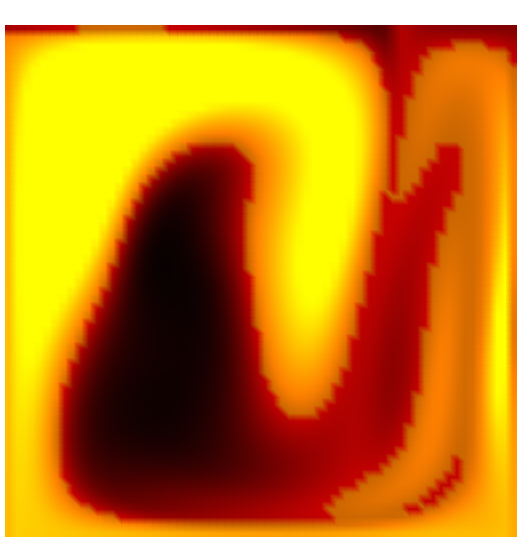
\includegraphics[width=0.3\textwidth]{images/demo}
\end{figure}

Implementing the demo gave me a great understanding of how things like velocity effect the simulation.
In the demo it is possible to toggle viewing the velocity on and off which greatly aided in my understanding of how the densities are propogated around the environment.

The fluid solver is very stable and I would recommend its use in 3D games.
It's big-oh complexity is known and is very acceptable, especially considering it is stable as other techniques for simulating fluids are not.
